% Introduce Iot, wireless sensor nodes, microrobot controllers, OpenWSN
% Go over currenet wireless sensor node solutions (and their shortcomings) focusing on the HW used for OpenWSN
% Talk about signle chip mote project, side-by-side HW/SW development for OpenWSN and other IoT applications
% This work is a starting point/foundation for the hardware, requires further development to reach the ideal/optimal solution
% Present repliminary results for power/timing/area, compare to current OpenWSN hardware
% Talk about future HW development work and upcoming tapeout
% Introduce the rest of the document

%<fancy hook shit>
%<talk about microrobots>
The term ``Smart Dust'' was originally coined by Professor Kris Pister to describe low-cost, low-maintenance, and unobtrusive wireless sensor nodes on a micro scale. These motes form interconnected mesh networks to communicate with one another and transmit sensor information. Sprinkling this dust over a field, on a road, or inside an office could provide valuable sensor data for a variety of applications... until the dust is swept away or thrown in the trash. On the other hand, mobile dust, in the form of autonomous microrobots, would be built with special MEMS devices that enable them to crawl or even fly. A swarm of these microrobots could space themselves out within a target area for optimal coverage, reposition themselves to areas with better wireless connectivity or illumination for their solar cells, or even mount a rescue for their brethren trapped within the depths of a Roomba.

While these ideas may appear to be more suited for science-fiction than reality, graduate students in Professor Pister's research group at UC Berkeley are actively designing MEMS structures for the purposes of microrobot movement and flight. However, before these robots can take their first tiny steps or fly off the surface of a lab bench, they will need a small but fully-functioning wireless sensor node for control and communication. The Single Chip Mote project aims to design an autonomous wireless sensor node with all external components integrated onto a single IC, without sacrificing the functionality needed for controlling swarms of microrobots.

\subsubsection{Wireless Sensor Nodes and the Internet of Things}
%<introduce IoT and wireless sensor nodes>
The recent rise in the popularity of the ``Internet of Things'' (IoT) has fueled the demand for consumer-quality wireless sensor node devices. While the availability and variety of these nodes continues to grow, the increasing popularity of IoT devices brings forth challenges in low-power communication and interoperability. The wireless standards used in laptops and cell phones such as WiFi and LTE are too power-hungry to be used on small wireless sensor nodes. Bluetooth Low Energy is appealing due to its compatibility with laptops and cell phones, at the cost of the associated licensing fees. It also does not support the creation of mesh networks. IEEE Standard 802.15.4, entitled Low-Rate Wireless Personal Area Networks, is also a popular choice since it defines the PHY and MAC layers underlying many other protocols commonly found on commercial motes. This standard is designed specifically for short-range, low-power, and low-data-rate application, and does not require licensing.

%<introduce OpenWSN>
The OpenWSN project \cite{openwsn} aims to create an open-source implementation of the complete protocol stack for IoT wireless sensor nodes with 802.15.4 radios. OpenWSN is compatible with a variety of software and hardware platforms, allowing different motes to communicate with one another and form mesh networks. Many of the top contributors to this project are former students and visiting scholars from Professor Pister's research group, and Professor Pister himself considers OpenWSN the ideal software platform for controlling and communicating with swarms of autonomous microrobots.

\subsubsection{When Small is Not Small Enough}
A quick overview of commercially-available wireless sensor nodes shows that many of these general-purpose motes have 8, 16, or 32-bit microprocessors running at frequencies on the order of 1-100MHz, 802.15.4 compliant radios, and a variety of inputs and outputs for analog and digital sensors. With these specifications, the motes are certainly capable of running OpenWSN and other applications within a mesh network. Their power consumption tends to be on the order of 1mW-1W while awake, requiring a battery or USB power. While these motes are small, able to fit within the palm of a hand, the weight of the battery and PCB itself makes them too large and heavy to be used for microrobotic control and communication. Without the benefit of energy harvesting, these motes also need to have their batteries replaced every few days or perhaps weeks. Examples of these motes include the TelosB and OpenMote-CC2538, both with OpenWSN support \cite{openwsn-hw}.

Research projects involving low-power motes tend to focus more on cramming commercial hardware onto tiny PCBs than in new embedded architectures for low-power applications. The designs presented in \cite{eco}, \cite{energy}, and \cite{transportation} are coin-sized, low-power, and unobtrusive motes optimized for infant observation, energy sensing, and transportation monitoring. And yet, all three are remarkably similar: a small 8-bit microprocessor, one or more PCBs stacked on top of one another, a coin-cell battery, and radio duty-cycling for energy savings. These motes perform the same main function as well: sample, transmit, sleep, and repeat. Given the simplicity of their microprocessors, these motes are not able to implement a complex protocol stack for mesh networks. \cite{eco} and \cite{transportation} also require their own base stations to communicate with the motes, whereas motes using IEEE 802.15.4 radios can communicate with any other mote or base station with an 802.15.4 transceiver. While these designs succeed in lowering energy consumption, they still require batteries that may only last for a few weeks, and the combination of the PCB and battery is still too heavy for a microrobot.

The authors of \cite{japan} claim to have developed the world’s smallest wireless sensor node by designing a custom IC for their signal processing and data transmission. The custom IC die is directly bonded to a MEMS die containing all of the required sensors. This mote still requires an external antenna, which is fabricated using a thin flexible substrate instead of a PCB. The mote uses solar cells in combination with a rechargeable battery for longer battery life; it can also run without a battery as long as there is sufficient illumination. This mote is small, lightweight, and has minimal external components. However, the major downside of the design in \cite{japan} is the lack of a general-purpose microprocessor, as it is designed for the sole purpose of sampling and transmitting data.

Perhaps the best attempt thus far towards full integration is the Michigan Micro Mote \cite{mmm}, a series of thin layers stacked like LEGOs in order to form a complete wireless sensor node.  With as many as eight different layers containing the microprocessor, radio, sensors, and other components, the mote measures at just $2 \times 4 \times 4 mm^3$, and has an incredibly low standby current of $2nA$. The mote can be powered completely via ambient light through its solar cells, and contains a battery layer to store any excess harvested energy. The only potential downside to this design is the increased complexity when manufacturing, aligning, and bonding eight different dies. This problem would only get worse when integrating microrobots into the design, as this would require a ninth layer for the robot body.

Finally, the 24/60GHz passive radio designed here at Berkeley \cite{ali-radio} proves that a low-power radio relying entirely on energy harvesting is possible on a single die. Unfortunately, the chip relies on energy scavenging from a high power RF source, and this asymmetric communication link means that the chip behaves more like an RFID tag instead of an autonomous computer. As a result, two of these radios cannot directly communicate with one another, and are not well-suited for forming a network of microrobots. Also, both the 24GHz receiver and 60GHz transmitter are not compliant with any current IoT standards.

\subsubsection{Single Chip Mote to the Rescue}
The Single Chip Mote project intends to combine the generality and processing capability of these not-so-small commercial sensor nodes with the lightweight form factor and low-power techniques used in the tiny, specialized wireless sensor nodes. The high-level block diagram in Figure \ref{fig:Mote} shows the various subsystems that must be integrated onto a single die in order for this project to succeed. While this project is still a work in progress, the final version of the Single Chip Mote will contain a fully-functional 32-bit ARM Cortex-M0 microprocessor, a low-power 2.4GHz IEEE 802.15.4 compatible radio, energy-harvesting solar cells, and an on-chip oscillator to create an autonomous wireless sensor node on a single CMOS die (or possibly a CMOS die bonded to a MEMS die). Without the need for any external components, a battery, or a PCB, the Single Chip Mote is the ideal microcontroller for the future swarms of autonomous microrobots, each with a lightweight yet fully-capable brain for performing actions beyond the simple observe and report. The addition of the OpenWSN protocol stack allows for these robots to create an extensive and adaptive mesh network, and communicate with a variety of IoT hardware platforms and sensors supporting OpenWSN.

\begin{figure}
\centering
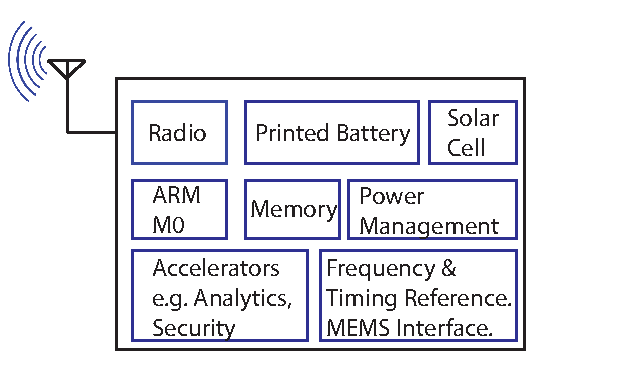
\includegraphics[width=0.7\linewidth]{/Mote}
\caption{High-level block diagram of the Single Chip Mote and its subsystems}
\label{fig:Mote}
\end{figure}

\subsubsection{Single Chip Mote Digital System}
The work presented in this report lays out the foundation for the digital components of the Single Chip Mote. A tested and functioning FPGA prototype of the Single Chip Mote digital system complete with an ARM Cortex-M0 microprocessor, radio controller, custom radio timer, and ADC interface is presented, along with the tools and procedures for designing hardware, writing software, and verifying functionality. A high-level block diagram of the Single Chip Mote digital system is shown in Figure \ref{fig:block-diagram}. This is far from the final iteration of the Single Chip Mote digital system; the design lacks support for integrated sensors, periodic sensing without intervention from the microprocessor, power management and low-power modes, and other potential hardware accelerators to handle repetitive and energy-consuming tasks normally executed in software.  As an example of hardware acceleration, OpenWSN uses hardware timers to wake up the microprocessor for each step involved in sending a packet over the radio (such as copying packet data, turning on the radio, telling the radio to send, listening for a response). The current Single Chip Mote digital system has custom timers designed to automatically trigger the actions required to send a packet without waking up the microprocessor, and the overall process requires less energy than a traditional microcontroller. The continuation and success of this project depends on the collaboration between digital designers and embedded systems developers in identifying potential processes that can be more efficiently carried out in hardware.

\begin{figure}
\centering
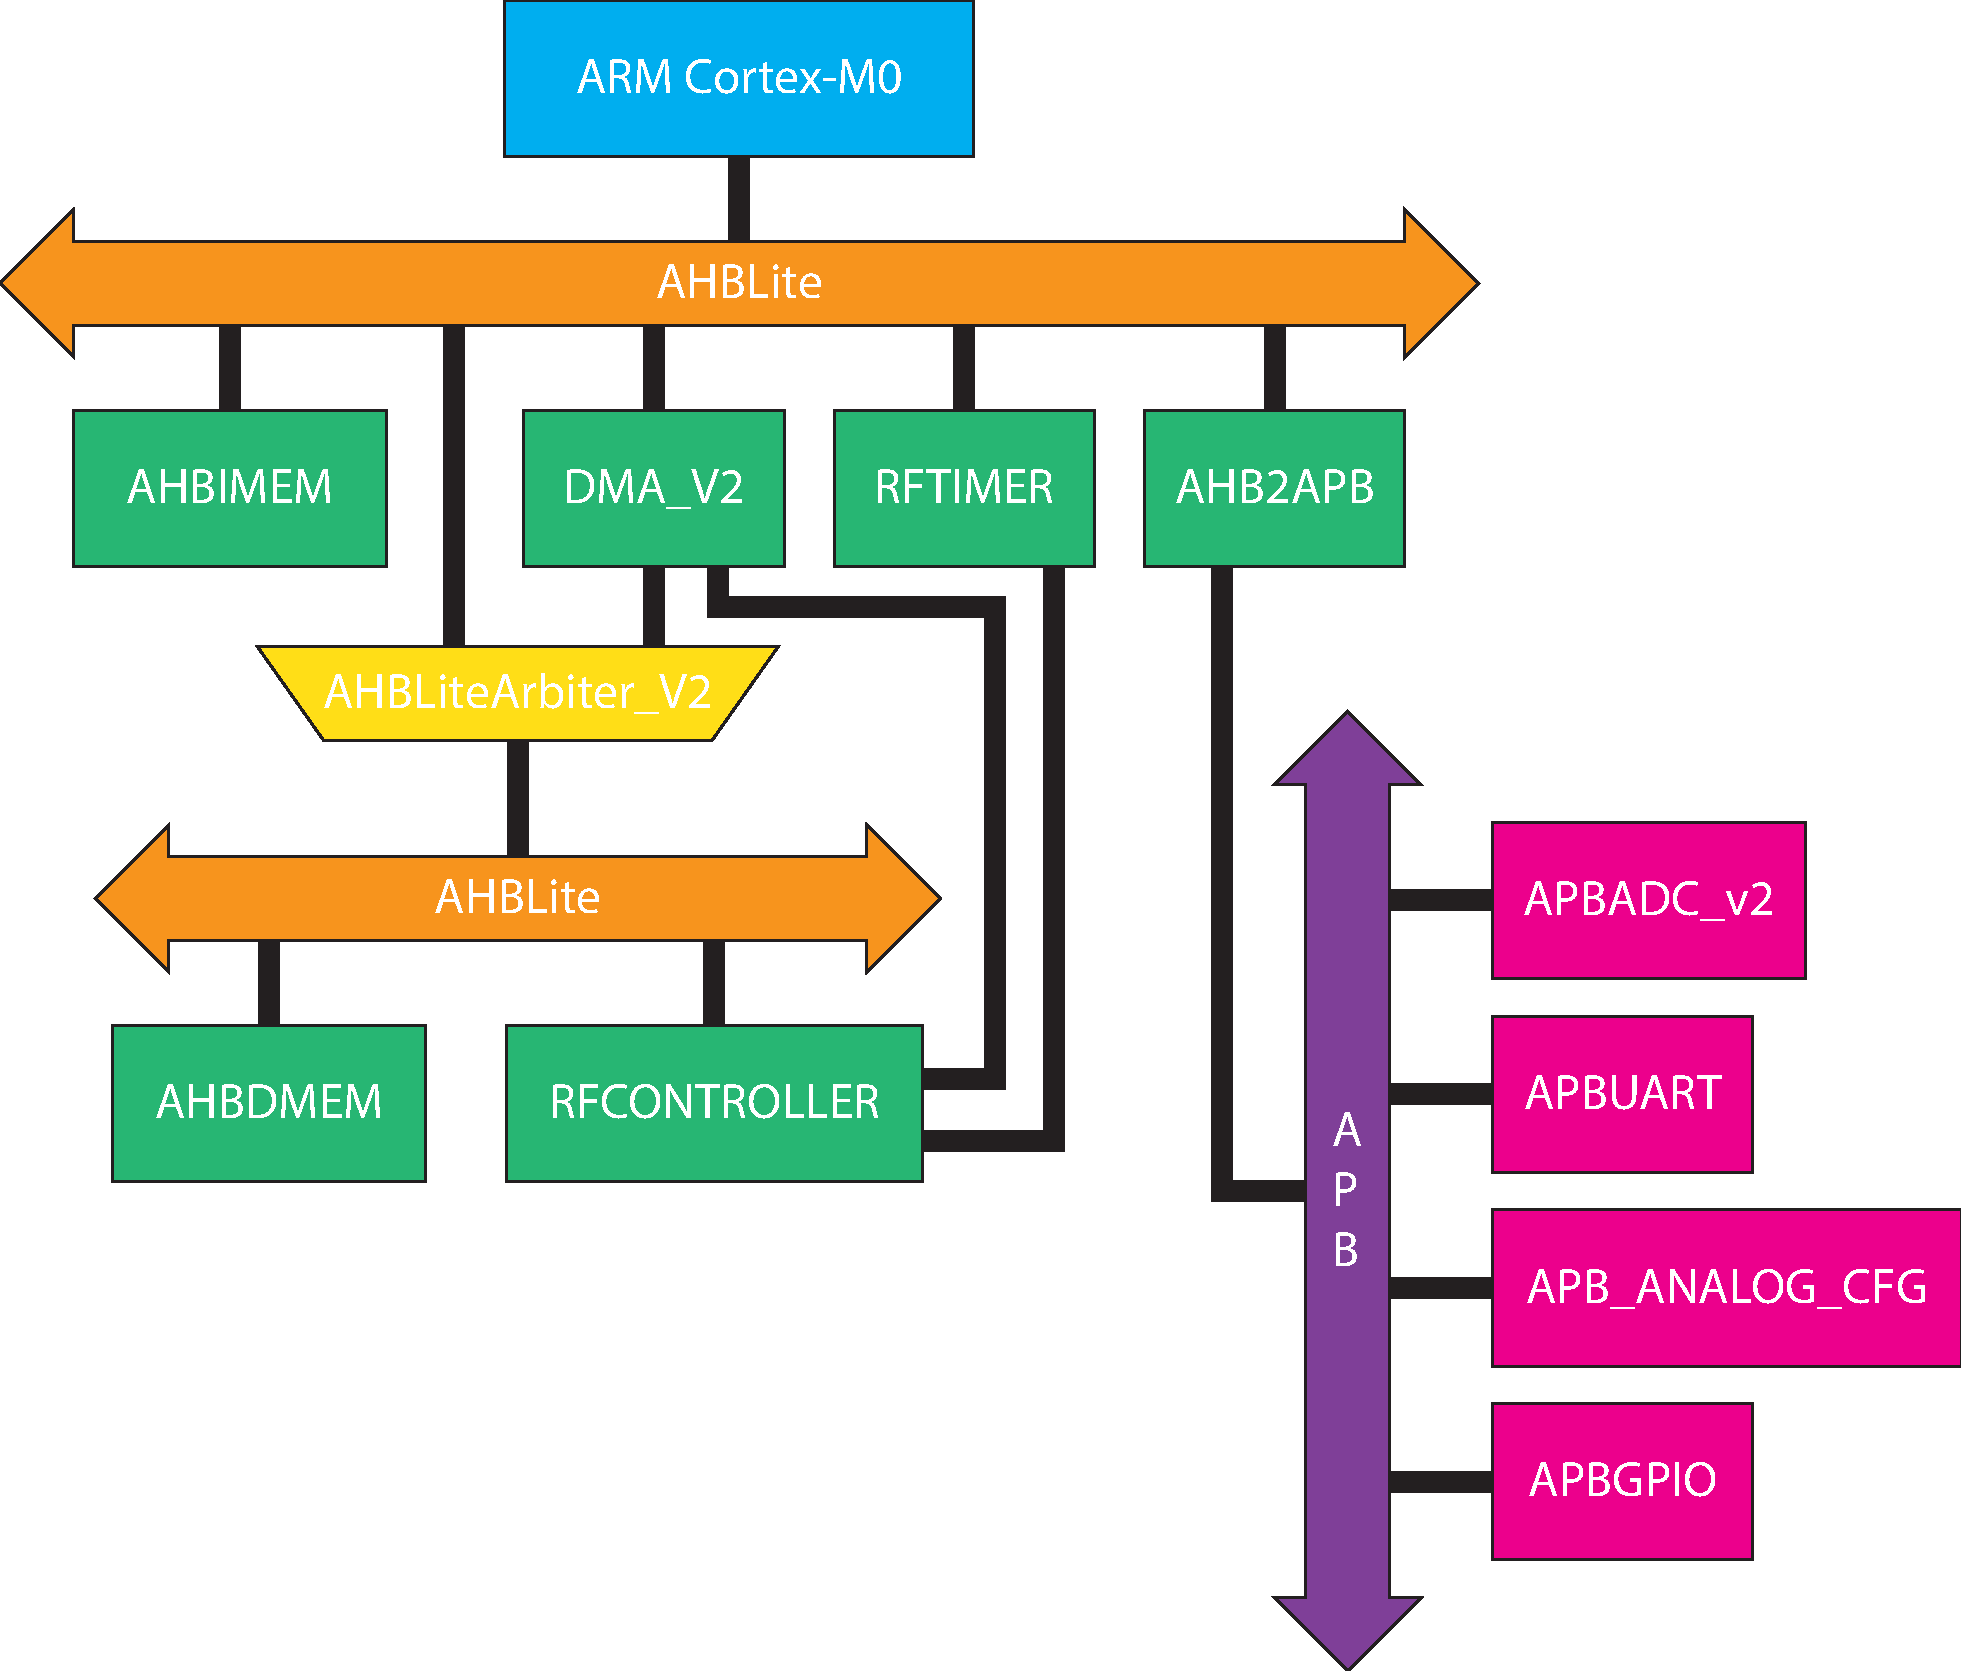
\includegraphics[width=0.7\linewidth]{block-diagram}
\caption{High-level block diagram of the Single Chip Mote digital system}
\label{fig:block-diagram}
\end{figure}

\subsubsection{Preliminary Results}
Preliminary results already show the potential for improvement when using the Single Chip Mote in place of existing wireless sensor nodes. Using the Verilog code described in this report, the Single Chip Mote digital system was synthesized, placed, and routed using Synopsys Design Compiler and Synopsys IC Compiler to obtain estimates for the area, power, and timing characteristics. Figure \ref{fig:M065nmLP} shows an image of the complete design. The technology used for this design is TSMC $65nm$ LP, with a clock frequency of $5MHz$ and an operating voltage of $1.2V$. The synthesis scripts are constrained to use only high threshold voltage (HVT) standard cells to reduce leakage current. While the digital system requires a additional debug hardware and improved floorplanning before tapeout, these initial results provide a more accurate estimate for evaluating this design relative to the goals of the project.

\begin{figure}
\centering
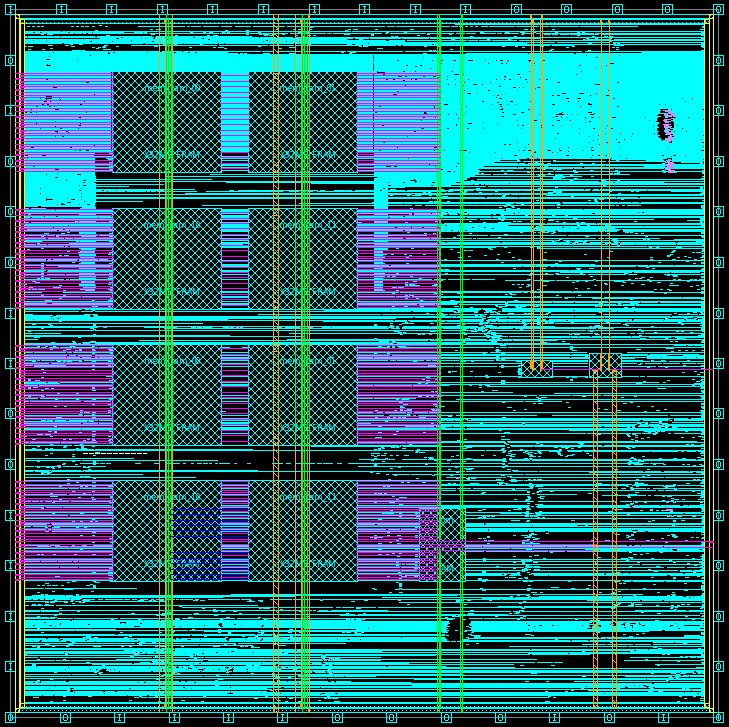
\includegraphics[width=0.7\linewidth]{M065nmLP}
\caption{Preliminary layout for the Single Chip Mote digital system}
\label{fig:M065nmLP}
\end{figure}

% Talk about LP process, HVT transistors, list area, power, and timing
%<describe the synthesis P&R, and results here>.
The target clock period of $200ns$ ($5MHz$ clock frequency) is relatively slow in a $65nm$ process, as evidenced by the ample critical path slack of $182ns$. While this design could easily run at faster clock frequencies, $5MHz$ was chosen in order to reduce dynamic power in the digital domain, as well as the power required by the on-chip oscillator for clock generation.

The dynamic power for this design is $139\mu W$, and the leakage power is $17.8\mu W$. These values are calculated using an operating voltage of $1.2V$, and can be further improved by scaling down the operating voltage. The LP (low-power) process was chosen since its high-threshold transistors significantly reduce leakage current. The main cost is that operating voltages are typically higher than in GP (general-purpose) processes in order to have the same on-current and run at similar speeds. However, since the Single Chip Mote digital system has a relatively slow clock frequency, it is acceptable to operate these transistors at a lower operating voltage and still meet timing requirements. Since dynamic power scales with $V_{dd}^2$, reducing the operating voltage to $0.9V$ reduces the dynamic power to $78.3\mu W$. Since leakage power scales with $V_{dd}$, reducing the operating voltage to $0.9V$ reduces the leakage power to $13.4\mu W$. Therefore, at $0.9V$, the Single Chip Mote digital system has a power budget of $91.7\mu W$. Reducing voltage requires that the standard cells are re-characterized at $0.9V$, since this information is not provided by TSMC.

The initial Single Chip Mote design does not have any power management hardware, clock gating, or power gating. Therefore, this design does not have any low power modes like the commercial microprocessors. However, the leakage power represents the power consumed when the Cortex-M0 is idle or asleep, and the sum of dynamic and leakage power indicates the power consumed while the Cortex-M0 is active. These results can be compared to the active and idle power consumption of commercial motes. The future addition of power gating to the Single Chip Mote will allow for more direct comparison to the low power modes of commercial microcontrollers. Also note that the power consumption reported does not include the radio or any additional hardware outside of the digital system.

One of the more popular microcontroller boards used for OpenWSN is the TelosB. This board contains the TI MSP430 microcontroller, which has an input voltage range of $1.8V$ to $3.6V$, and an active current of $330\mu A$ at $1MHz$ and $2.2V$, according to the datasheet \cite{msp430}. These measurements indicate an active power of $726\mu W$. The datasheet does not specifically state the current draw while the CPU is idle, but it does have the current draw for four of the five low power modes: $50\mu A$, $11\mu A$, $1.1\mu A$, and $0.2\mu A$. These low power modes use clock gating, power gating, and powering down oscillators to reduce current draw. At $2.2V$, the resulting power for each of the measured low power modes is $110\mu W$, $24.2\mu W$, $2.42\mu W$, and $0.44\mu W$. The active power of the Single Chip Mote digital system is much smaller than that of the MSP430, while still running at a higher frequency. Although the MSP430 low power modes cannot be directly compared to the idle power of the Single Chip Mote, it is clear that the Single Chip Mote, without any clock or power gating, has lower power while idle than the MSP430 does in its first low power mode.

Another board developed specifically for OpenWSN development is the OpenMote-CC2538, which uses the TI CC2438 microcontroller. According to the datasheet \cite{cc2538}, the CC2538 has an input voltage range of $2V$ to $3.6V$, and its current draw varies based on which peripherals are active. The current draw while the CPU is running and clocked with an RC oscillator (and the radio, crystals, and peripherals are turned off), is $7mA$. The datasheet does not list the current draw while idle, but it does have three low power modes implemented using clock gating, power gating, and powering down oscillators. These three low power modes have a current draw of $0.6mA$, $1.3\mu A$, and $0.4\mu A$. Assuming an input voltage of $2V$ is used, the power while active is $14mW$, and the power during the three low power modes is $1.2mW$, $2.6\mu W$, and $0.8\mu W$. The active power of the Single Chip Mote digital system is much smaller than that of the CC2538. Although the CC2538 low power modes cannot be directly compared to the idle power of the Single Chip Mote, it is clear that the Single Chip Mote, without any clock or power gating, has lower power while idle than the CC2538 does in its first low power mode.

While these numbers are optimistic, the main reason for the improvement is most likely due the use of the $65nm$ LP processes. The Single Chip Mote digital system also has significantly fewer on-chip peripherals than the MSP430 or CC2538, reducing both dynamic and leakage power. The CC2538 also uses an ARM Cortex-M3 processor, which requires more power when compared to the ARM Cortex-M0. 

Area is also an important consideration, since this chip must be light enough to be carried by a MEMS microrobot. The preliminary design for the Single Chip Mote digital system has a total cell area of $856600\mu m^2$, which easily fits within a die area of $1mm^2$. Assuming an incident power of $1mW$ per $mm^2$ in direct sunlight, CMOS solar cells with at least $10\%$ conversion efficiency should be able to provide $100\mu W$ per $mm^2$ of die area in direct sunlight. Therefore, this design (when run with an operating voltage $0.9V$) requires approximately $1mm^2$ of solar cells to power the Single Chip Mote digital system. It is estimated that the analog, radio, and voltage converters for the Single Chip Mote will require $2mm^2$ of area for the circuits themselves, and $2mm^2$ of area for additional solar cells. With these numbers in mind, the Single Chip Mote requires a total die area of $6mm^2$. Given that the thickness of the die is about $200\mu m$, and the density is similar to that of crystalline silicon ($2.33g/cm^3$), the estimated mass of the die is $2.8mg$.

Researchers in our group are currently designing MEMS motors and legs for walking microrobots. Each leg outputs a downward force of $300\mu N$, and can move a mass of $30mg$. The mass of the legs themselves are $15mg$ each, which allows for $15mg$ of payload per leg. With these values in mind, a one-legged MEMS microrobot generates enough downward force to support the weight of the Single Chip Mote.


\subsubsection{Future Work}
%<talk about tapeout here>
While the RTL design of the preliminary Single Chip Mote digital system is complete, there is still more work required before the Single Chip Mote is ready for widespread use. The Single Chip Mote team submitted a tapeout in March 2016 containing the first version of the analog and radio circuits, which will be fabricated and tested in May 2016. Building off of the results of the first tapeout, the team is targeting a second tapeout in August 2016, which will include the first version of the digital system (as described in this report) and the second version of the analog and radio circuits. The results of this second tapeout, as well as feedback from software developers from the OpenWSN project, will determine the direction of this project in 2017 and beyond.

\subsubsection{Report Outline}
%<introduce the rest of the document>
The rest of this report covers the details of the Single Chip Mote digital system design, as well as the development tools and testing procedures. Chapter \ref{getting-started} provides an overview of the tools for hardware development for the FPGA and software development for the Cortex-M0 microprocessor, including the basics of their installation and use. Chapter \ref{hw} contains a detailed explanation of the Single Chip Mote digital system hardware, and chapter \ref{sw} demonstrates how to write software that uses the hardware peripherals. Chapter \ref{bootloading} covers the details on loading software onto an FPGA or ASIC containing the Single Chip Mote digital system. Chapter \ref{testing} describes the current testing procedures, including simulation and real-time verification. Chapter \ref{transitioning-to-asic} details the changes required to convert the Single Chip Mote digital system from an FPGA design to an ASIC design. Chapter \ref{conclusion} concludes this report with a discussion the accomplishments of this project and areas for improvement. The bibliography beginning on page \pageref{bib} contains a list of the references included in this report.
